\documentclass{standalone}
\usepackage{standalone}

\begin{document}
\subsection{Experiment with SVM}
As we stated before support vector machine draws a straight line between two class. That's why it always perform well in two class.First of all, we transform the whole data set into TfidfVectorizer. We set kernel='linear', set idf, penalty parameter C=1 and kernel coefficient gamma=1. We trained our data set for age and got result with performance 25\% accuracy which was very low. Because the age class has eight features that are 18,19,20,21,22,23,24,25. We also trained our data set with SVM for religion class. Our religion class has 4 features with ratio that are Muslim 61.4\% , Hindu 35.2\% , Christian 1.1\% and Buddist 2.3\%. We got performance  76.36\% accuracy. We tried our best to keep our data set in equal ratio. But due to lack of sufficient user we were unable to do that. In the other we trained our data set with sex class that has only two features that are Male or Female. Our model perform very well with 87.5\% accuracy. We can say that this accuracy is significant. We also trained our model for both Sex and Age that performed with 34.61\% accuracy which is not significant. Table-5.3 shows all  accuracy in percentage.
\begin{table}[h]
	\centering
	\begin{tabular}{|c|c|c|}
		\hline
		\begin{tabular}[c]{@{}c@{}}Category\\ \end{tabular} & \begin{tabular}[c]{@{}c@{}}Accuracy\\ (\%)\end{tabular} & \begin{tabular}[c]{@{}c@{}}Decision\\ \end{tabular} \\ \hline
		 Age & 25\% &  Not good\\ \hline
		 Sex and Age & 34.61\% &  Not good\\ \hline
		 Religion & 76.36\% & Good \\ \hline
		 Sex & 87.5\% & Significant \\ \hline
	\end{tabular}
	\caption{ Accuracy of SVM.}
	\label{tab:error5}
\end{table}

\begin{figure}[h]
				\centering
				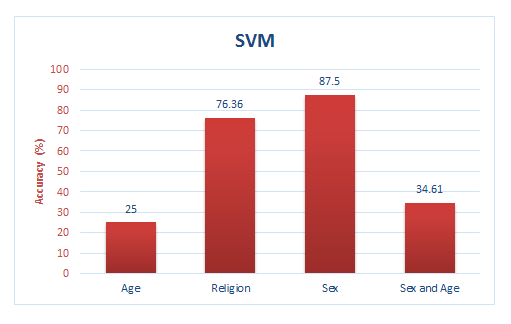
\includegraphics[scale=0.8]{./img/SVM1}
				\caption{Performance diagram with SVM} \label{fig:mapComp}
\end{figure}
  

\end{document} 